
\documentclass{article}
\usepackage{graphicx} % Required for inserting images
\usepackage{caption} % Required for \captionof
\usepackage{amsmath}
\usepackage{float}
\usepackage{comment}
\usepackage[T1]{fontenc}
\usepackage[utf8]{inputenc}
\usepackage{lmodern}
\usepackage{microtype}
\usepackage{xcolor}
\usepackage{framed}
\renewenvironment{leftbar}{%
  \def\FrameCommand{\textcolor{orange}{\vrule width 3pt} \hspace{10pt}}%
  \MakeFramed {\advance\hsize-\width \FrameRestore}}%
 {\endMakeFramed}

\title{Mechanikai mérés}
\author{Kern Luca, Vincze Csongor}
\date{2026 Április 22}

\begin{document}

\maketitle

\section*{4. Feladat: Igazolja a Steiner-tételt!}


\vspace{0.5em}
\noindent
\textbf{Mérési adatok és paraméterek:} \\
$m_{\text{piros csap}} = 2,08 \text{ kg}$ \\[1ex]


\vspace{1em}
\noindent


\begin{figure}[H]
    \centering
    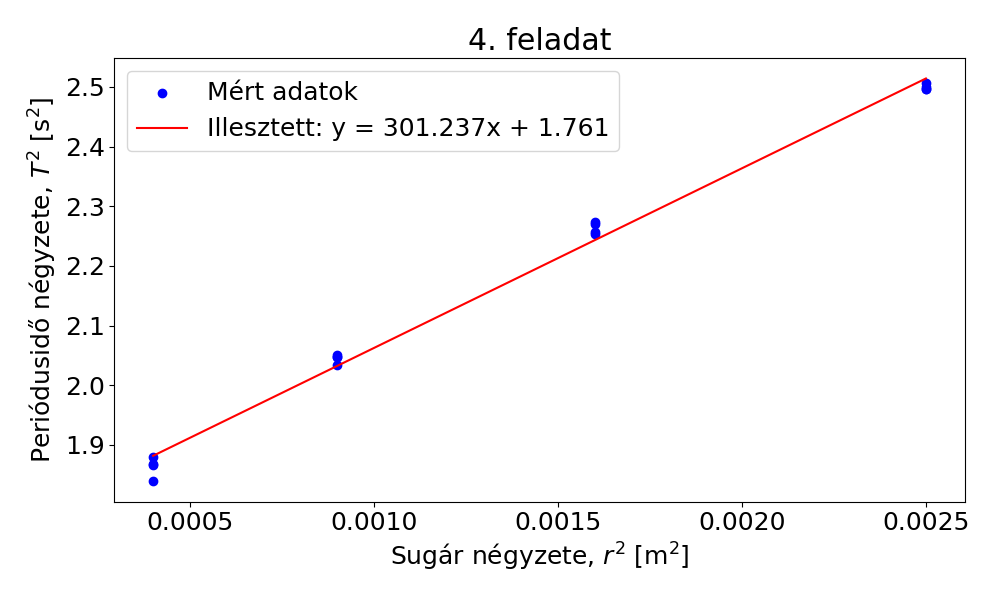
\includegraphics[width=0.8\textwidth]{../images/4_feladat.png}
    \caption{A mérési adatok és az illesztett egyenes a Steiner-tétel igazolásához}
    \label{fig:4}
\end{figure}

A direkciós állandóra $k^{*} = 6,74 \cdot 10^{-3} \text{ Nm}$ adódott. A tehetetlensegi nyomatekra pedig $ 2.8 \cdot 10^{-4} \text{kg m^2}$

\end{document}
